\documentclass[11pt]{amsart}

% Encoding and fonts
\usepackage[T1]{fontenc}
\usepackage[utf8]{inputenc}
\usepackage{lmodern}

% Math packages
\usepackage{amsmath}
\usepackage{amssymb}
\usepackage{amsfonts}
\usepackage{amsthm}
\usepackage{mathtools}

% Figures and layout
\usepackage{graphicx}
\usepackage{geometry}
\usepackage{enumitem}
\usepackage[hidelinks]{hyperref}

\geometry{margin=1in}

\numberwithin{equation}{section}
\setcounter{tocdepth}{3}
\setcounter{secnumdepth}{3}

% ---------------------------------------------------------
% Theorem-like environments
% ---------------------------------------------------------

\theoremstyle{plain}
\newtheorem{theorem}{Theorem}[section]
\newtheorem{proposition}[theorem]{Proposition}
\newtheorem{lemma}[theorem]{Lemma}
\newtheorem{corollary}[theorem]{Corollary}
\newtheorem{conjecture}[theorem]{Conjecture}

\theoremstyle{definition}
\newtheorem{definition}[theorem]{Definition}
\newtheorem{experiment}[theorem]{Experiment}
\newtheorem{heuristic}[theorem]{Heuristic}
\newtheorem{question}[theorem]{Question}

\theoremstyle{remark}
\newtheorem{remark}[theorem]{Remark}
\newtheorem{warning}[theorem]{Warning}

\title{A Vector and Mellin--Functional Route from a Mertens Walk to a Symmetrized \texorpdfstring{$\xi$}{xi}-Family}
\author{}
\date{}

\begin{document}

\maketitle

\tableofcontents

\bigskip

\begin{remark}
\label{rem:exploratory_nature}
This notebook is exploratory in nature.  It records a chain of ideas starting from numerical phase-walk pictures of the Mertens function and a squarefree correction, and ending with a proposed Mellin--functional family built from the completed zeta function.  Statements labelled as lemmas or propositions are intended as formal or conditional statements.  Statements labelled as heuristics, experiments, warnings, or open problems are not proofs of the Riemann hypothesis.
\end{remark}

\section{Motivation from phase-walk geometry}
\label{sec:motivation_phase_walk_geometry}

The initial object was not a Dirichlet series but a geometric walk.  The ordinary Mertens function is
\begin{equation}
M(x)=\sum_{n\leq x}\mu(n),
\label{eq:mertens_definition}
\end{equation}
where \(\mu\) is the M\"obius function.  The numerical pictures motivating this notebook considered the growth of a walk over Mertens, with an added real component coming from the squarefree counting error.

\begin{figure}[htbp]
\centering
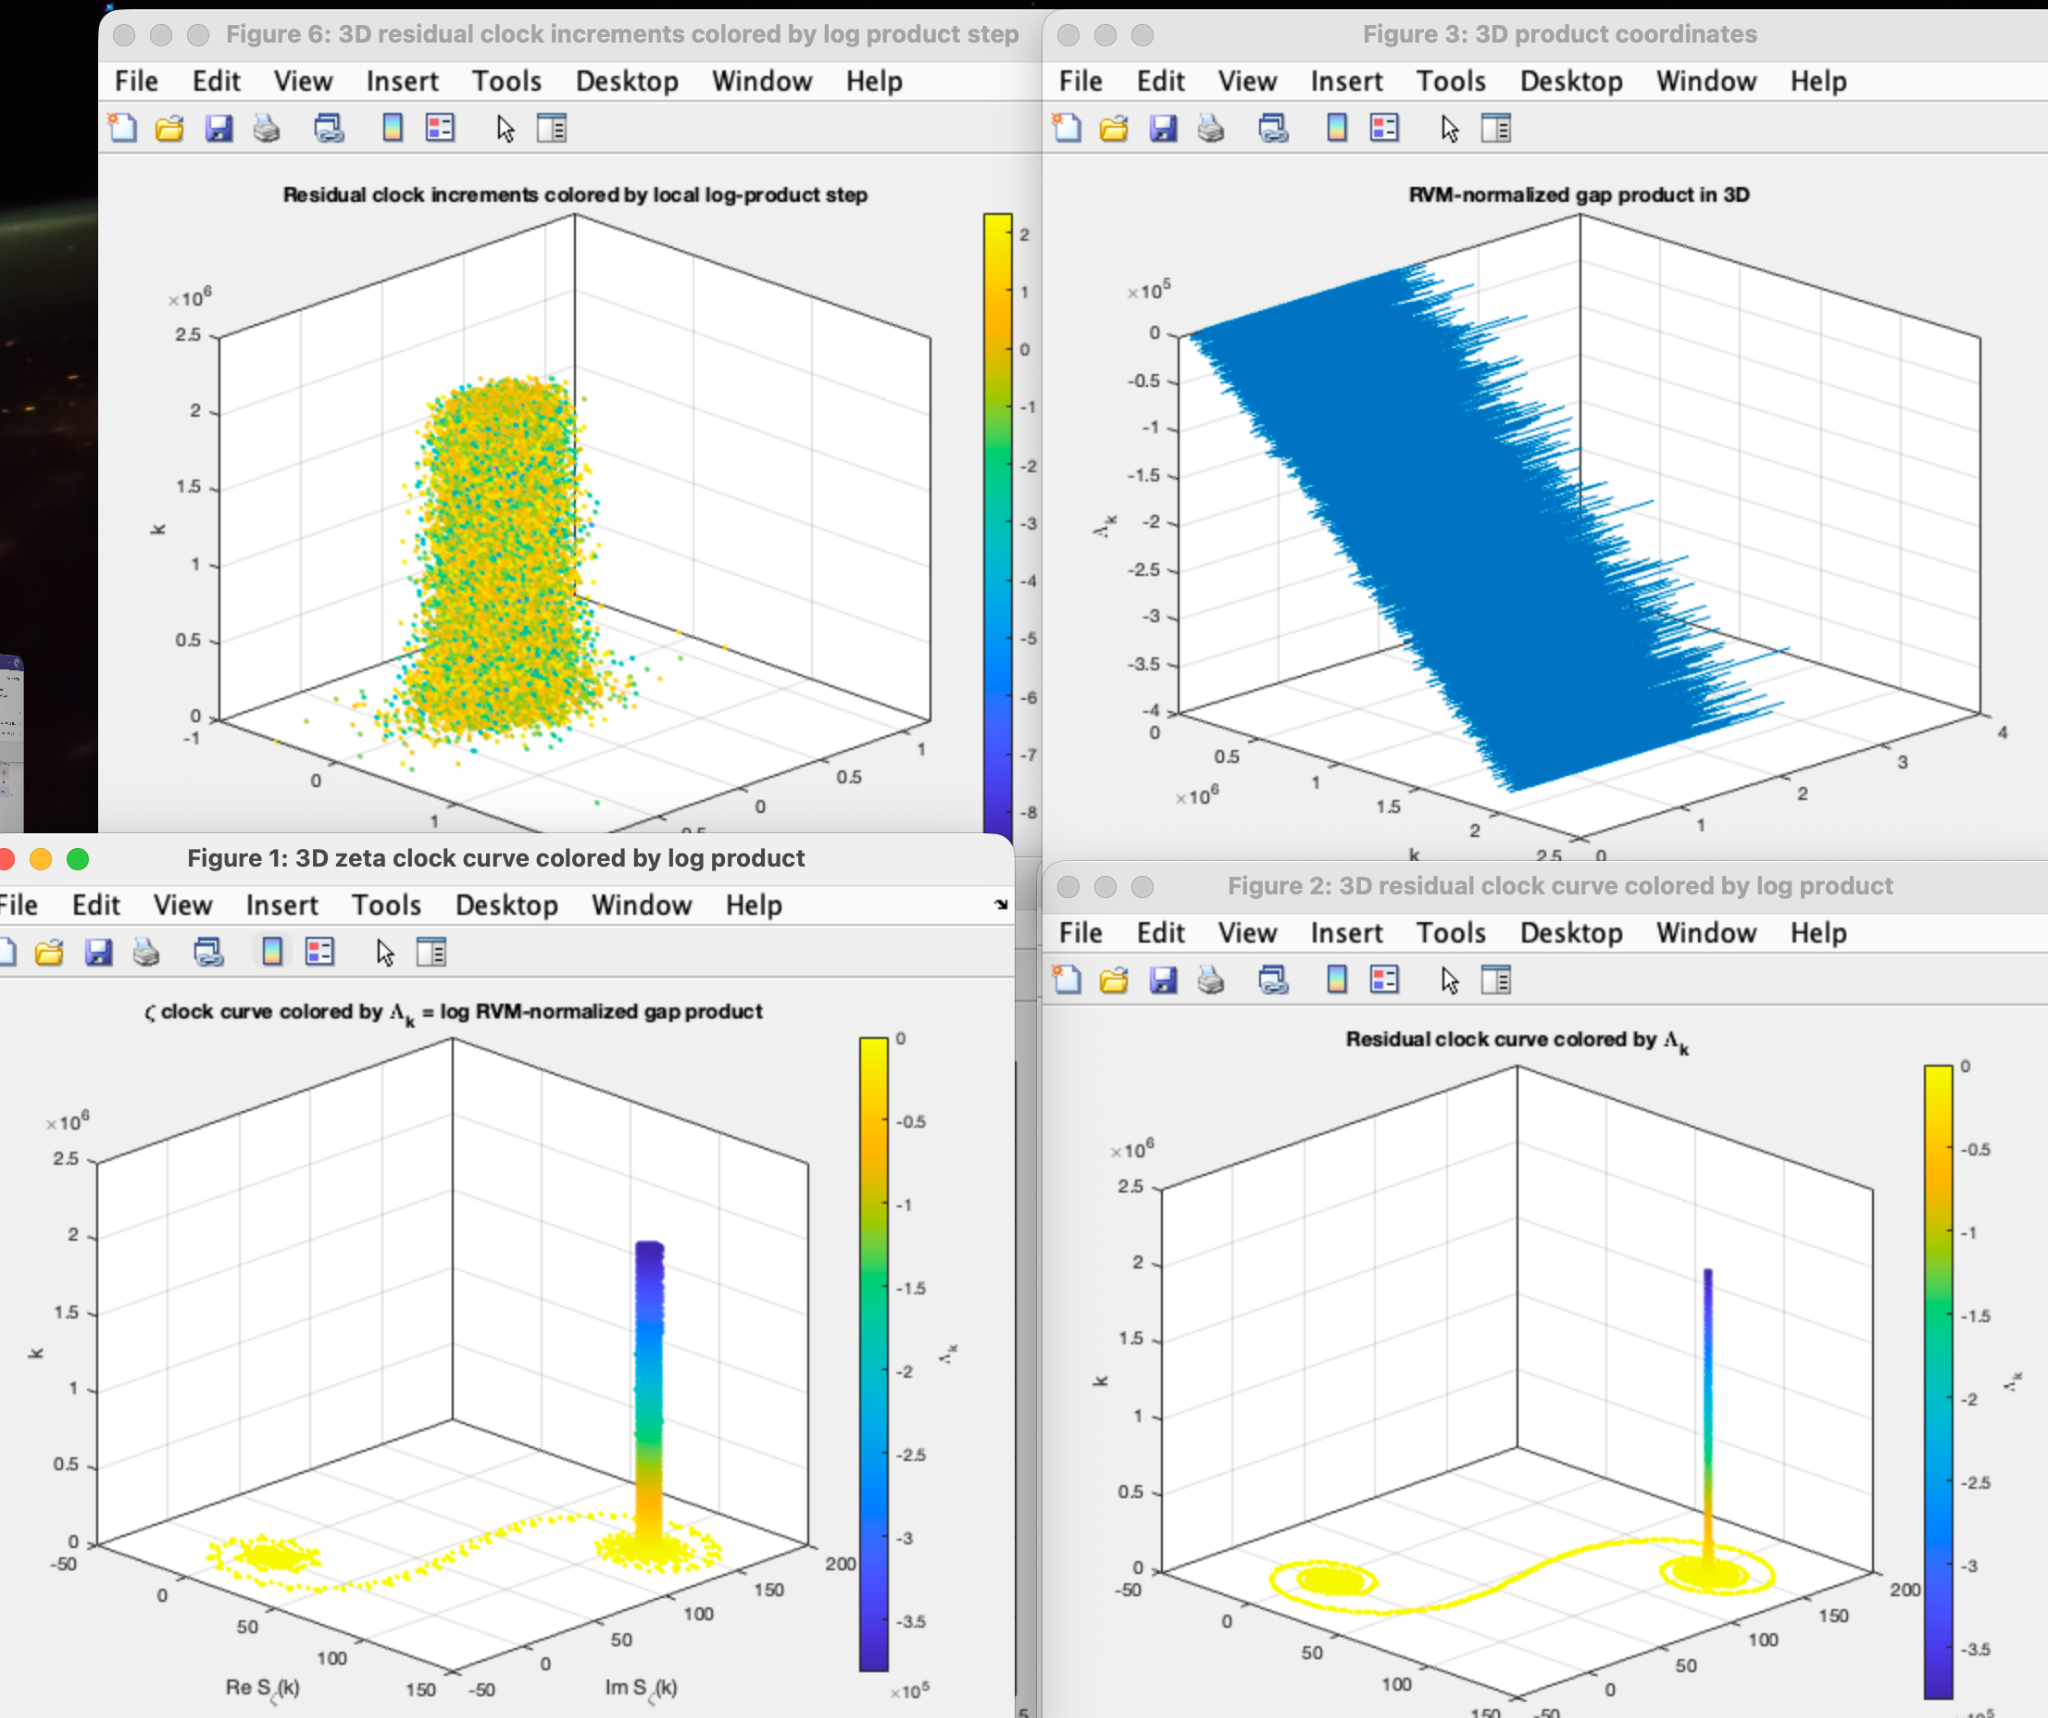
\includegraphics[width=0.96\textwidth]{figures/fig_749.png}
\caption{Uploaded numerical phase-walk figures.  The relevant qualitative observation is the growth of a three-dimensional cloud or surface when the Mertens walk is augmented by a second arithmetic component.  This figure is used only as motivation, not as evidence for a theorem.}
\label{fig:phase_walk_3d_motivation}
\end{figure}

\begin{figure}[htbp]
\centering
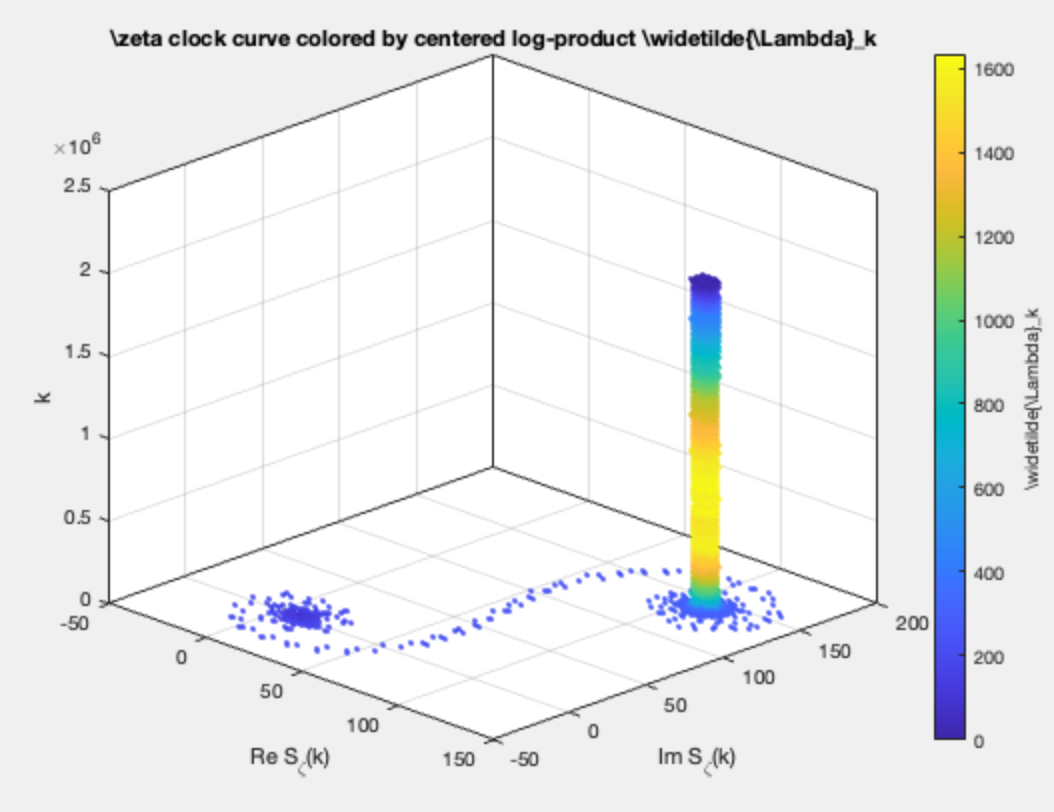
\includegraphics[width=0.72\textwidth]{figures/fig_752.png}
\caption{Uploaded centered/log-product three-dimensional visualization.  The figure motivates an anisotropic viewpoint: the Mertens axis and the squarefree-error axis need not have the same natural scaling.}
\label{fig:centered_log_product_3d}
\end{figure}

\begin{figure}[htbp]
\centering
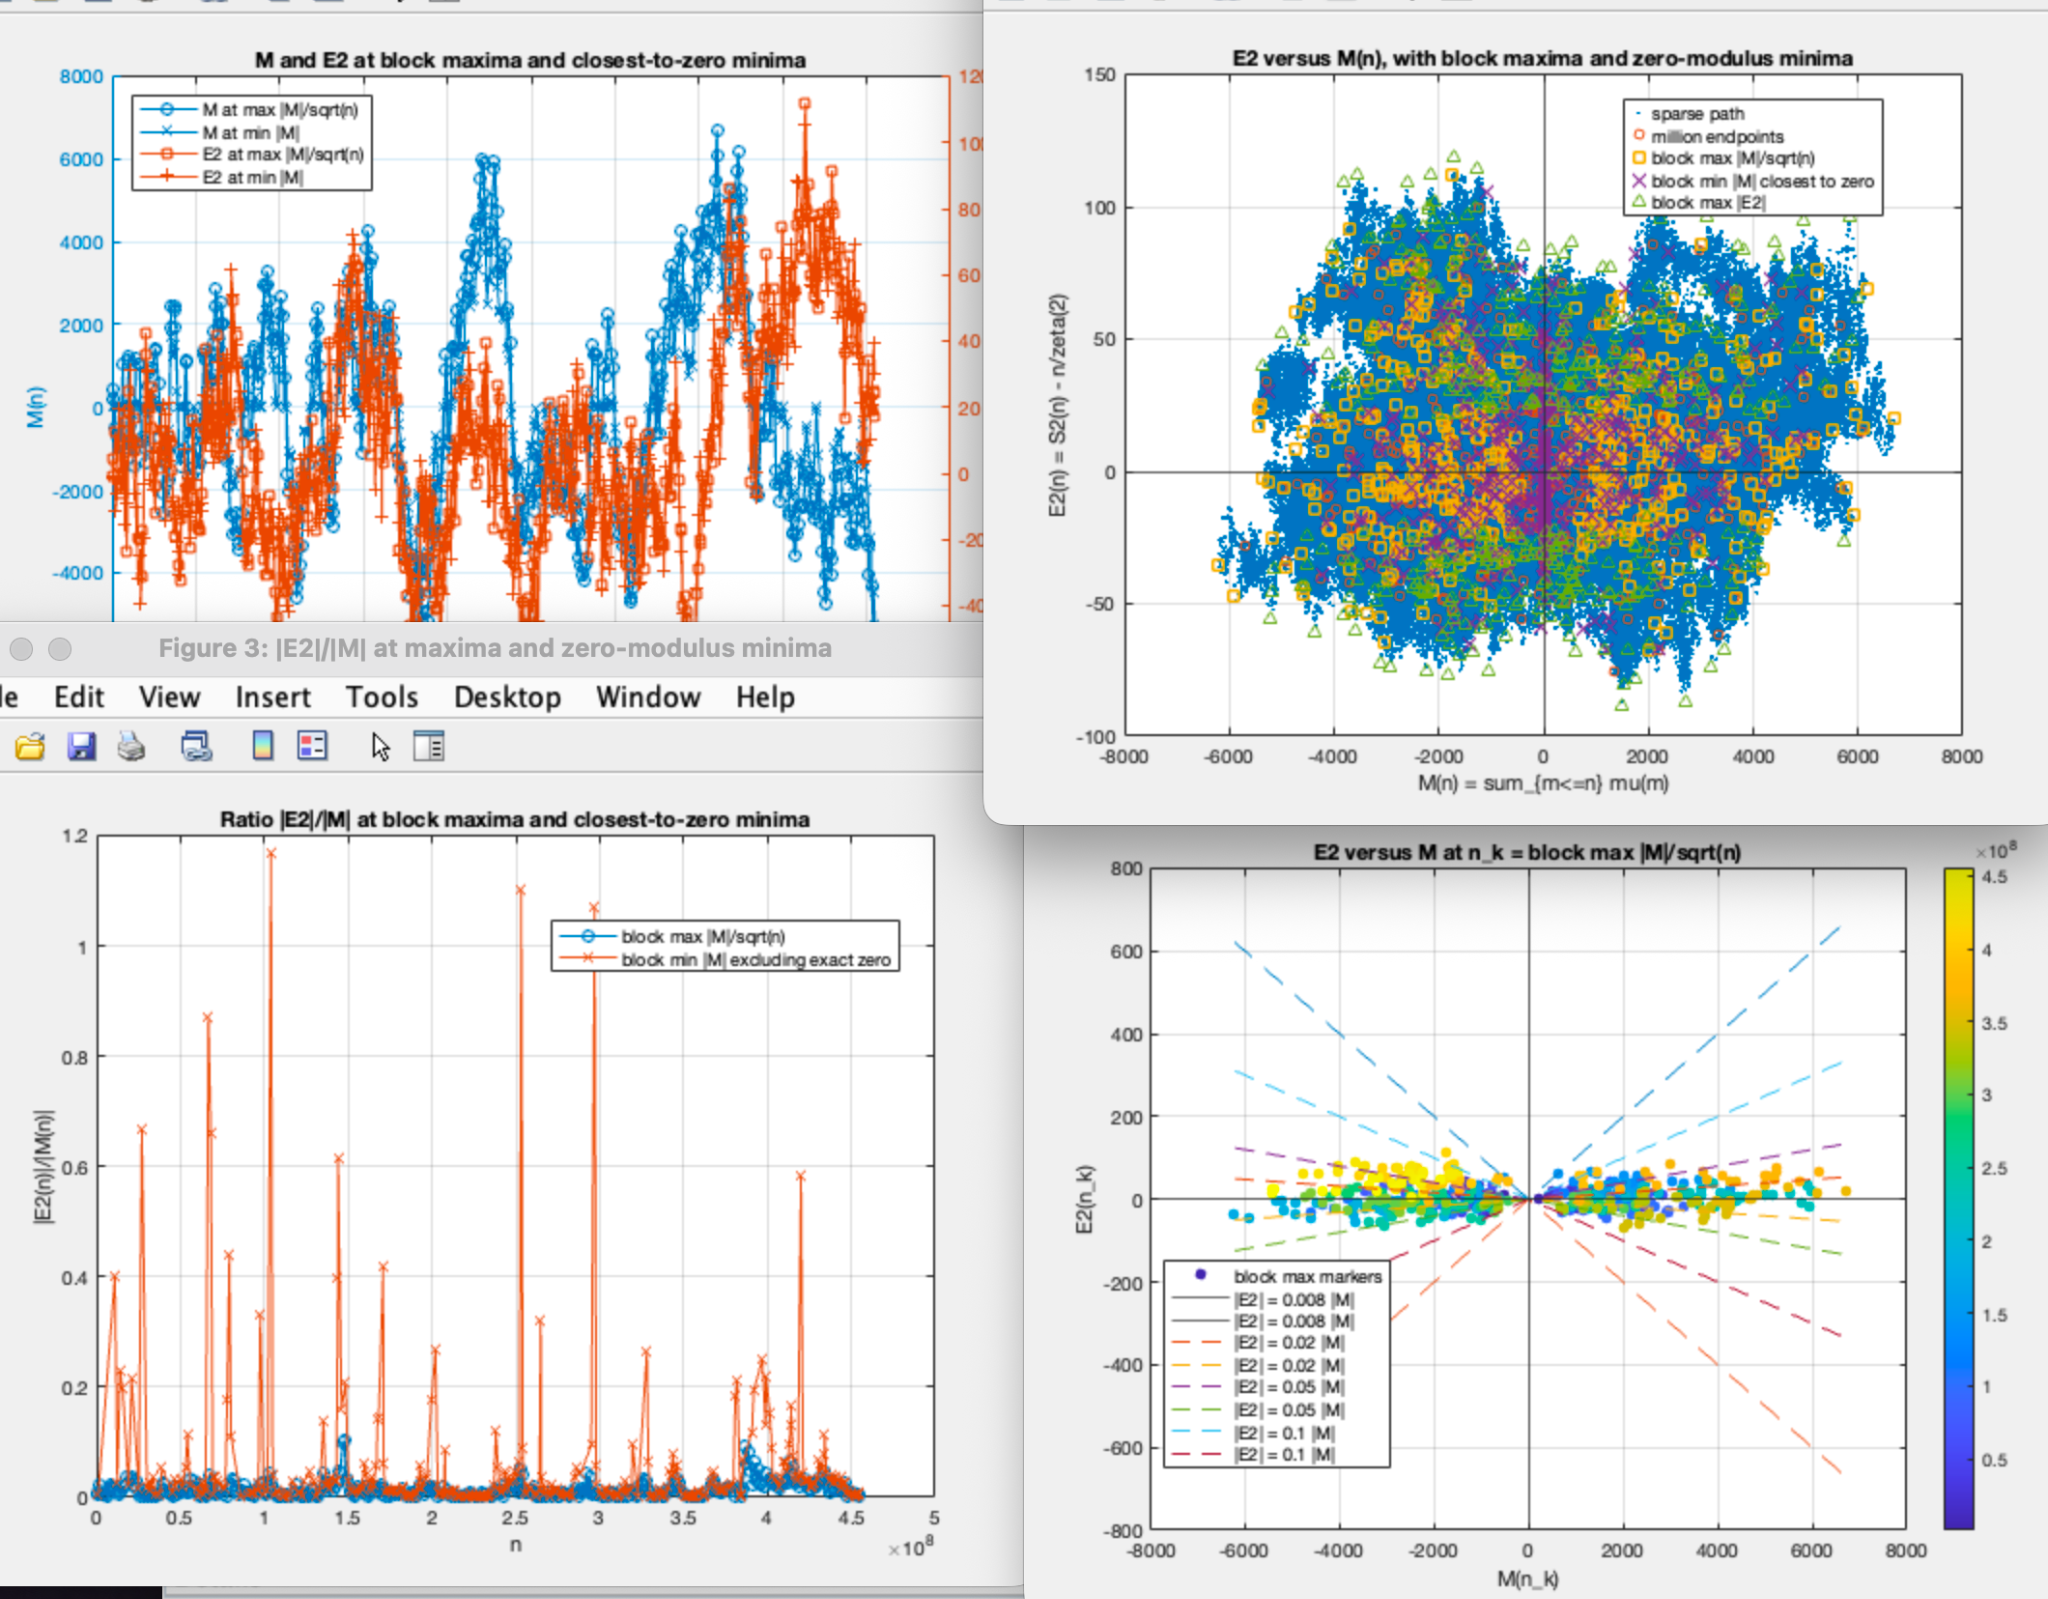
\includegraphics[width=0.96\textwidth]{figures/fig_765.png}
\caption{Uploaded numerical comparison panels from the Mertens and squarefree-error experiments.  The panels are treated here as computational observations only.}
\label{fig:mertens_squarefree_panels_one}
\end{figure}

\begin{figure}[htbp]
\centering
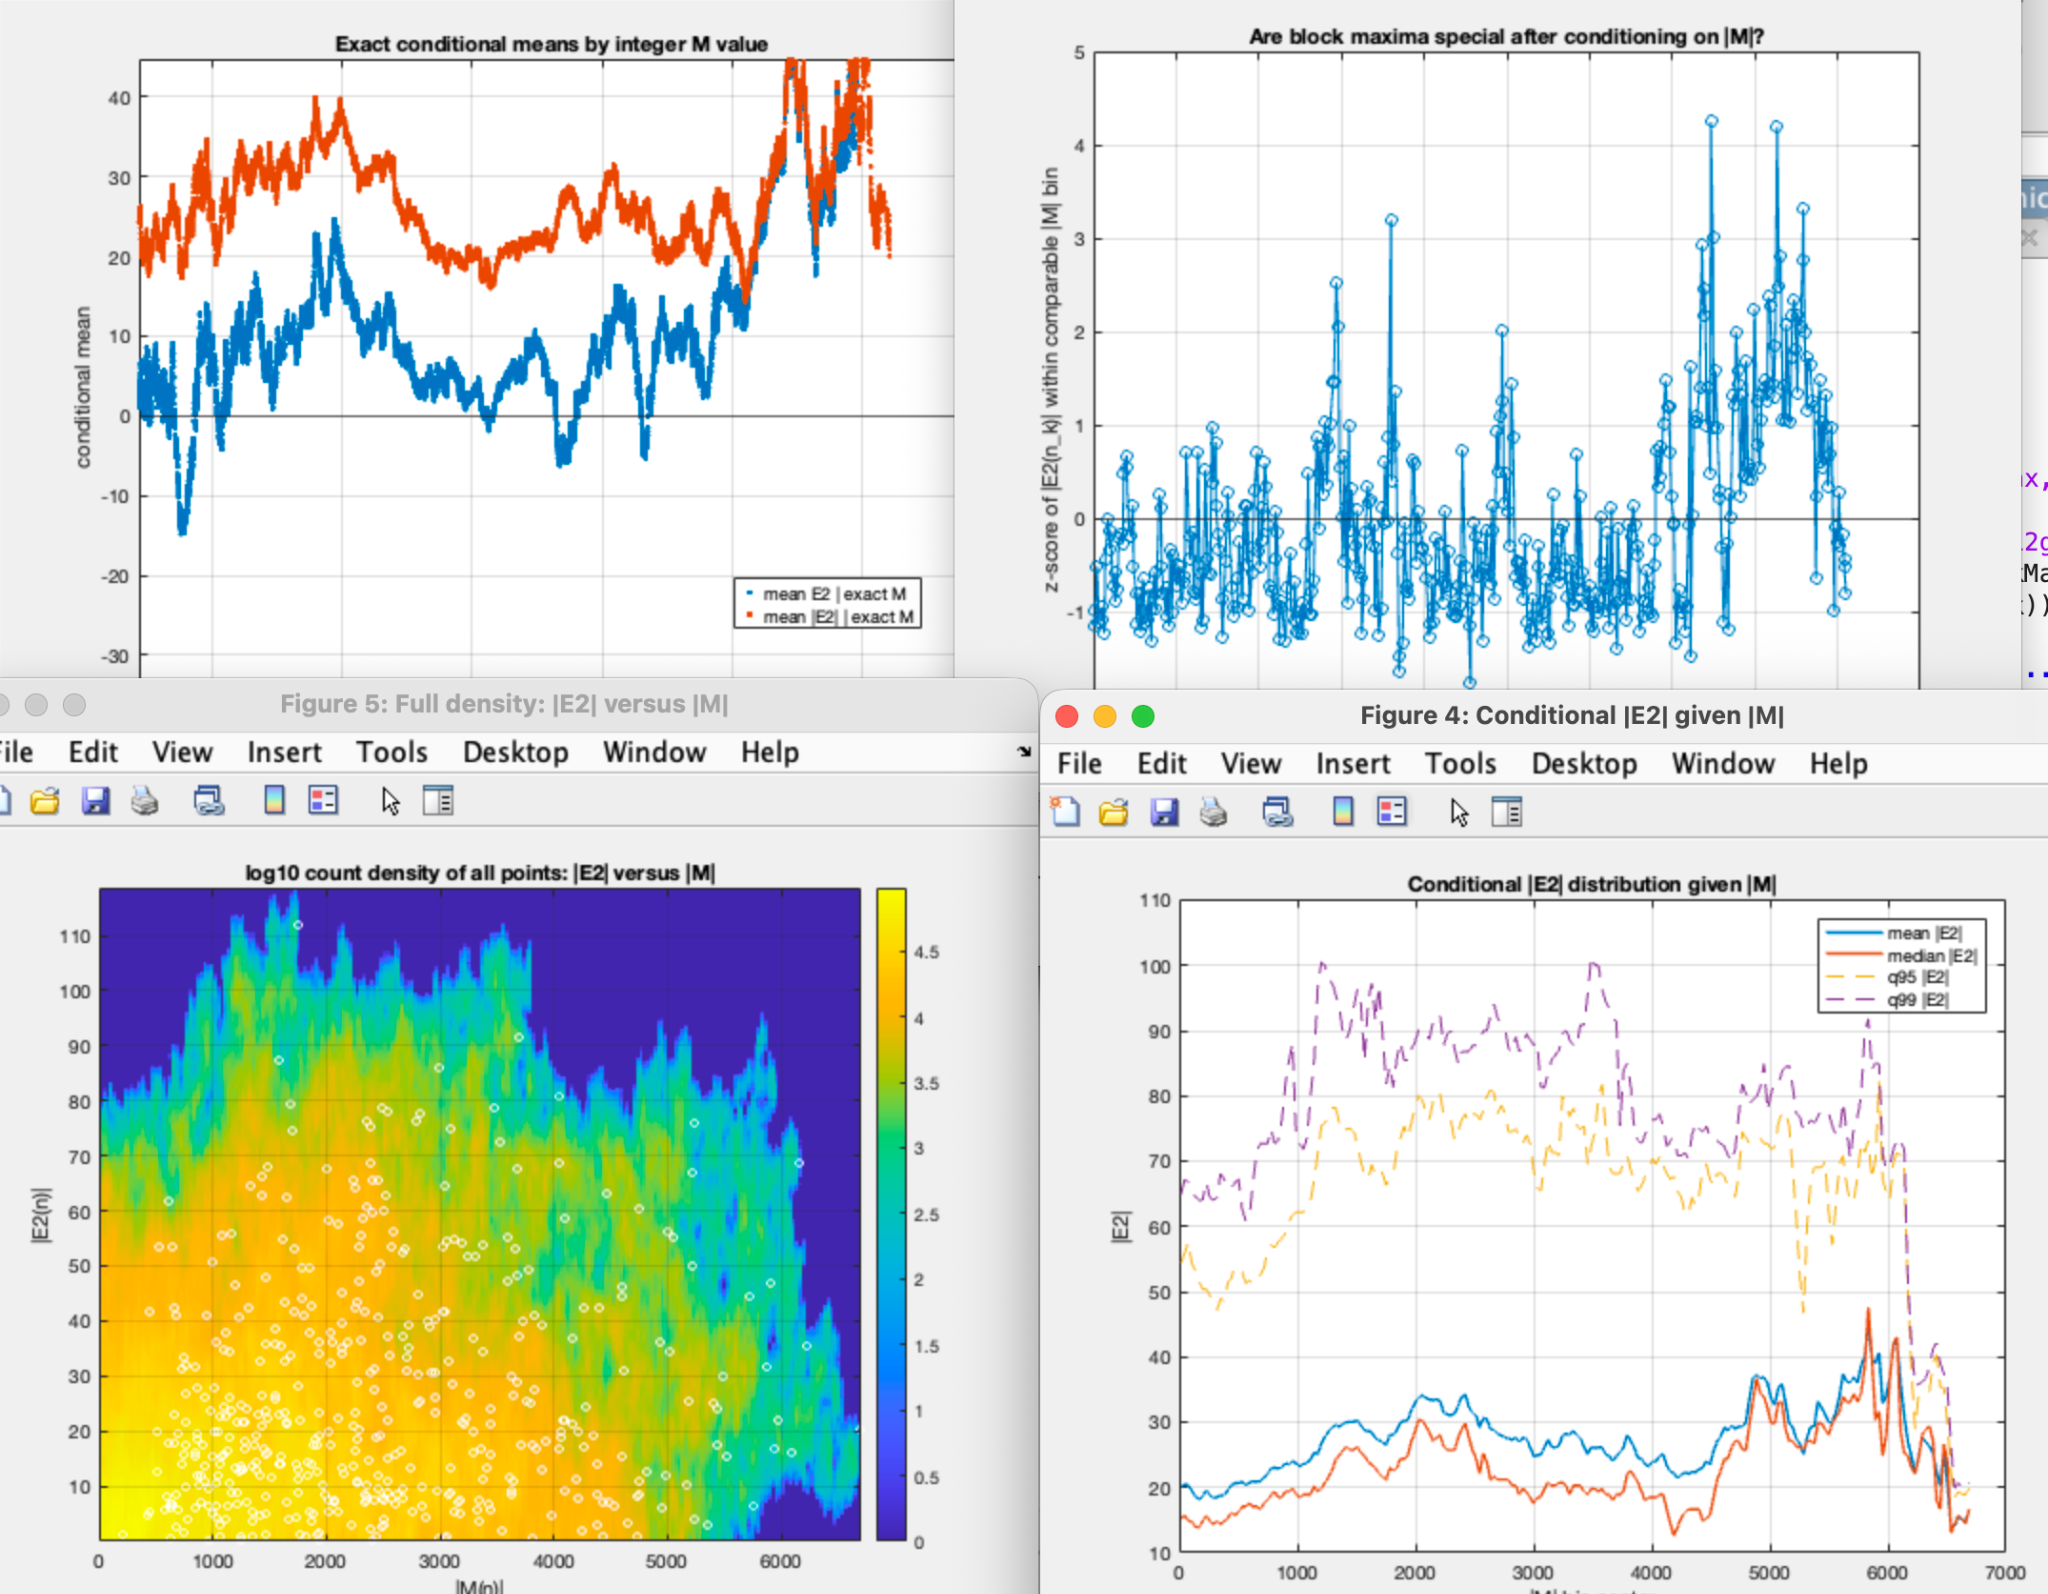
\includegraphics[width=0.96\textwidth]{figures/fig_766.png}
\caption{Uploaded numerical comparison panels from the later geometric investigation.  These images motivate the search for a two-channel analytic formulation rather than a single Euclidean norm.}
\label{fig:mertens_squarefree_panels_two}
\end{figure}

\begin{experiment}
\label{exp:computational_starting_point}
The computational logs used a file containing \(455,052,511\) values of \(\mu(n)\).  In the million-by-million scan the endpoint was reported at
\begin{equation}
N=455,052,511,
\qquad
M(N)=-5414,
\qquad
\theta_{\mathrm{end}}\approx 0.251833^{\circ},
\label{eq:experiment_endpoint_values}
\end{equation}
and the fitted endpoint angle statistic was reported in the form
\begin{equation}
\tan\theta(N)\approx A N^b,
\qquad
A\approx 0.2089756943,
\qquad
b\approx -0.145023366.
\label{eq:experiment_angle_fit}
\end{equation}
These numerical values are recorded as exploratory data.  They do not constitute a proof of any asymptotic statement.
\end{experiment}

\section{The arithmetic two-channel object}
\label{sec:arithmetic_two_channel_object}

Let
\begin{equation}
S_2(x)=\sum_{n\leq x}\mu(n)^2
\label{eq:squarefree_count_definition}
\end{equation}
be the squarefree counting function.  Define the squarefree error by
\begin{equation}
E_2(x)=S_2(x)-\frac{x}{\zeta(2)}.
\label{eq:squarefree_error_definition}
\end{equation}
The centered real component used in the geometric walk may also be written with the opposite sign,
\begin{equation}
R(x)=\frac{x}{\zeta(2)}-S_2(x)=-E_2(x).
\label{eq:R_definition}
\end{equation}
The basic two-channel vector is therefore
\begin{equation}
Z_\mu(x)=R(x)+iM(x).
\label{eq:complex_mobius_vector}
\end{equation}
Equivalently, in terms of \(E_2\),
\begin{equation}
Z_\mu(x)=-E_2(x)+iM(x).
\label{eq:complex_mobius_vector_E2}
\end{equation}

\begin{remark}
\label{rem:anisotropic_scaling}
The natural scales of the two components are different.  The Mertens channel is associated with the critical scale \(x^{1/2}\), whereas the squarefree-error channel is associated with the scale \(x^{1/4}\) after the substitution \(x=t^2\).  This is the reason for considering \(M(t)\) and \(E_2(t^2)\) together.
\end{remark}

\begin{definition}
\label{def:direct_lambda_channel}
For a complex parameter \(\lambda\), define the direct combined channel by
\begin{equation}
C_\lambda(t)=M(t)+\lambda E_2(t^2).
\label{eq:C_lambda_definition}
\end{equation}
This is the direct, unsymmetrized arithmetic channel.
\end{definition}

\section{Dirichlet series and the direct family}
\label{sec:dirichlet_series_direct_family}

The standard Dirichlet series identities are
\begin{equation}
\sum_{n=1}^{\infty}\frac{\mu(n)}{n^s}=\frac{1}{\zeta(s)},
\qquad
\Re s>1,
\label{eq:mobius_dirichlet_series}
\end{equation}
and
\begin{equation}
\sum_{n=1}^{\infty}\frac{\mu(n)^2}{n^s}=\frac{\zeta(s)}{\zeta(2s)},
\qquad
\Re s>1.
\label{eq:squarefree_dirichlet_series}
\end{equation}
These are standard identities in analytic number theory; see \cite{Titchmarsh1986,IwaniecKowalski2004}.

The re-scaled squarefree channel is produced formally by
\begin{equation}
\frac{\zeta(s/2)}{\zeta(s)}
=\left(\sum_{a=1}^{\infty}a^{-s/2}\right)
\left(\sum_{b=1}^{\infty}\frac{\mu(b)}{b^s}\right).
\label{eq:rescaled_squarefree_dirichlet_product}
\end{equation}
Consequently, its summatory form is
\begin{align}
\sum_{a^{1/2}b\leq t}\mu(b)
&=\sum_{b\leq t}\mu(b)\left\lfloor \frac{t^2}{b^2}\right\rfloor
\label{eq:rescaled_squarefree_sum_floor}\\
&=S_2(t^2).
\label{eq:rescaled_squarefree_sum_squarefree}
\end{align}
Thus the centered direct family corresponds formally to
\begin{equation}
D_\lambda(s)=\frac{1}{\zeta(s)}
+\lambda\left(\frac{\zeta(s/2)}{\zeta(s)}-\frac{\zeta(s)}{\zeta(2)}\right).
\label{eq:D_lambda_definition}
\end{equation}

\begin{warning}
\label{warn:direct_family_is_change_of_coordinates}
The direct family \(C_\lambda\) alone is not a new analytic mechanism.  Two independent values of \(\lambda\) recover \(M(t)\) and \(E_2(t^2)\) by linear algebra.  The direct family is useful as a compact notation, but it is not by itself a proof strategy.
\end{warning}

\section{Known scales and the squarefree channel}
\label{sec:known_scales_squarefree_channel}

The error term in squarefree counting is a standard object.  Write
\begin{equation}
R_2(x)=S_2(x)-\frac{x}{\zeta(2)}.
\label{eq:R2_literature_definition}
\end{equation}
The general \(k\)-free error is often denoted
\begin{equation}
R_k(x)=Q_k(x)-\frac{x}{\zeta(k)}.
\label{eq:Rk_literature_definition}
\end{equation}
Mossinghoff, Oliveira e Silva, and Trudgian record the expected scale
\begin{equation}
R_k(x)=O_\varepsilon\left(x^{1/(2k)+\varepsilon}\right),
\label{eq:kfree_expected_scale}
\end{equation}
and prove large oscillation results and extensive computations for \(k=2,3,4,5\) \cite{MossinghoffOliveiraTrudgian2021}.  For \(k=2\), the expected scale is
\begin{equation}
R_2(x)=O_\varepsilon\left(x^{1/4+\varepsilon}\right).
\label{eq:squarefree_expected_scale}
\end{equation}

\begin{remark}
\label{rem:squarefree_channel_status}
Equation \eqref{eq:squarefree_expected_scale} is recorded as the natural squarefree-error scale.  This notebook does not claim a proof of \eqref{eq:squarefree_expected_scale}.  The purpose is to embed the squarefree channel into a vectorial analytic framework together with the Mertens channel.
\end{remark}

\begin{proposition}
\label{prop:direct_cota_would_be_strong}
Assume that both estimates
\begin{equation}
M(t)=O_\varepsilon\left(t^{1/2+\varepsilon}\right)
\label{eq:mertens_rh_scale_estimate}
\end{equation}
and
\begin{equation}
E_2(t^2)=O_\varepsilon\left(t^{1/2+\varepsilon}\right)
\label{eq:squarefree_rescaled_rh_scale_estimate}
\end{equation}
hold for every \(\varepsilon>0\).  Then, for every fixed \(\lambda\),
\begin{equation}
C_\lambda(t)=O_{\varepsilon,\lambda}\left(t^{1/2+\varepsilon}\right).
\label{eq:C_lambda_direct_bound}
\end{equation}
\end{proposition}

\begin{proof}
This follows immediately from \eqref{eq:C_lambda_definition}, \eqref{eq:mertens_rh_scale_estimate}, and \eqref{eq:squarefree_rescaled_rh_scale_estimate}.
\end{proof}

\begin{warning}
\label{warn:no_reverse_from_single_lambda}
A single estimate of the form \eqref{eq:C_lambda_direct_bound} for one value of \(\lambda\) does not recover separate estimates for \(M\) and \(E_2\).  Two independent values of \(\lambda\) recover the vector algebraically, but this is still a change of coordinates unless an additional analytic operation is introduced.
\end{warning}

\section{Replacing \texorpdfstring{$\zeta$}{zeta} by the completed function}
\label{sec:completed_function_replacement}

Define
\begin{equation}
A(s)=\frac12s(s-1)\pi^{-s/2}\Gamma(s/2),
\label{eq:A_definition}
\end{equation}
and
\begin{equation}
\xi(s)=A(s)\zeta(s).
\label{eq:xi_definition}
\end{equation}
The completed zeta function satisfies the functional equation
\begin{equation}
\xi(s)=\xi(1-s),
\label{eq:xi_functional_equation}
\end{equation}
which is standard; see \cite{Titchmarsh1986,Edwards1974,IwaniecKowalski2004}.

\begin{lemma}
\label{lem:xi_reversible}
Away from the explicitly known zeros and poles of the factor \(A(s)\), passing from \(\zeta(s)\) to \(\xi(s)\) is reversible.
\end{lemma}

\begin{proof}
Equation \eqref{eq:xi_definition} gives
\begin{equation}
\zeta(s)=\frac{\xi(s)}{A(s)}.
\label{eq:zeta_recovered_from_xi}
\end{equation}
Similarly,
\begin{equation}
\frac1{\zeta(s)}=\frac{A(s)}{\xi(s)}.
\label{eq:inverse_zeta_from_xi}
\end{equation}
Thus no information about the nontrivial zeros is lost by using \(\xi\), except for the already known factors in \(A(s)\).
\end{proof}

The two non-reflected components become
\begin{equation}
\frac1{\zeta(s)}=\frac{A(s)}{\xi(s)},
\label{eq:nonreflected_component_one}
\end{equation}
and
\begin{equation}
\frac{\zeta(s/2)}{\zeta(s)}=\frac{A(s)\zeta(s/2)}{\xi(s)}.
\label{eq:nonreflected_component_two}
\end{equation}
Using \eqref{eq:xi_functional_equation}, the reflected components are
\begin{equation}
\frac{A(1-s)}{\xi(s)},
\label{eq:reflected_component_one}
\end{equation}
and
\begin{equation}
\frac{A(1-s)\zeta((1-s)/2)}{\xi(s)}.
\label{eq:reflected_component_two}
\end{equation}

\begin{definition}
\label{def:xi_vector}
The completed vector family is
\begin{equation}
\mathcal V(s)=\frac1{\xi(s)}
\begin{pmatrix}
A(s)\\
A(s)\zeta(s/2)\\
A(1-s)\\
A(1-s)\zeta((1-s)/2)
\end{pmatrix}.
\label{eq:xi_vector_definition}
\end{equation}
\end{definition}

\begin{remark}
\label{rem:why_xi_vector_is_not_projective}
The vector \(\mathcal V(s)\) is not a projectivization.  Its first component is exactly \(1/\zeta(s)\) by \eqref{eq:nonreflected_component_one}.  Therefore a bound on the full vector would control the Mertens channel.  This is different from taking a quotient of two components, which would remove the scalar denominator and lose the size information.
\end{remark}

\section{The symmetrized \texorpdfstring{$\lambda$}{lambda}-family}
\label{sec:symmetrized_lambda_family}

For \(\lambda\in\mathbb C\), define the numerators
\begin{equation}
N_\lambda^{\pm}(s)=A(s)(1+\lambda\zeta(s/2))
\pm A(1-s)(1+\lambda\zeta((1-s)/2)).
\label{eq:N_lambda_pm_definition}
\end{equation}
The symmetrized functions are
\begin{equation}
F_\lambda^{\pm}(s)=\frac{N_\lambda^{\pm}(s)}{\xi(s)}.
\label{eq:F_lambda_pm_definition}
\end{equation}
Equivalently,
\begin{align}
F_\lambda^{+}(s)+F_\lambda^{-}(s)
&=2\frac{A(s)(1+\lambda\zeta(s/2))}{\xi(s)},
\label{eq:F_sum_recovers_nonreflected}\\
F_\lambda^{+}(s)-F_\lambda^{-}(s)
&=2\frac{A(1-s)(1+\lambda\zeta((1-s)/2))}{\xi(s)}.
\label{eq:F_difference_recovers_reflected}
\end{align}
Thus the pair \((F_\lambda^+,F_\lambda^-)\) contains both the original and reflected channels.

\begin{definition}
\label{def:PQ_pm}
Set
\begin{equation}
P^{\pm}(s)=A(s)\pm A(1-s),
\label{eq:P_pm_definition}
\end{equation}
and
\begin{equation}
Q^{\pm}(s)=A(s)\zeta(s/2)\pm A(1-s)\zeta((1-s)/2).
\label{eq:Q_pm_definition}
\end{equation}
Then
\begin{equation}
N_\lambda^{\pm}(s)=P^{\pm}(s)+\lambda Q^{\pm}(s).
\label{eq:N_as_P_plus_lambda_Q}
\end{equation}
\end{definition}

\begin{lemma}
\label{lem:lambda_one_i_detection}
If
\begin{equation}
N_1^{\pm}(s)=0
\qquad\text{and}\qquad
N_i^{\pm}(s)=0,
\label{eq:simultaneous_N_one_i_zero}
\end{equation}
then
\begin{equation}
P^{\pm}(s)=0
\qquad\text{and}\qquad
Q^{\pm}(s)=0.
\label{eq:simultaneous_PQ_zero}
\end{equation}
\end{lemma}

\begin{proof}
Using \eqref{eq:N_as_P_plus_lambda_Q}, the assumptions \eqref{eq:simultaneous_N_one_i_zero} are
\begin{equation}
P^{\pm}(s)+Q^{\pm}(s)=0,
\label{eq:linear_system_one}
\end{equation}
and
\begin{equation}
P^{\pm}(s)+iQ^{\pm}(s)=0.
\label{eq:linear_system_i}
\end{equation}
Subtracting \eqref{eq:linear_system_one} from \eqref{eq:linear_system_i} gives
\begin{equation}
(i-1)Q^{\pm}(s)=0.
\label{eq:Q_zero_from_two_lambdas}
\end{equation}
Since \(i-1\neq 0\), this gives \(Q^{\pm}(s)=0\).  Substitution into \eqref{eq:linear_system_one} gives \(P^{\pm}(s)=0\).
\end{proof}

\begin{warning}
\label{warn:numerators_not_enough}
Lemma \ref{lem:lambda_one_i_detection} is only an algebraic non-cancellation test.  It does not prove that \(F_1^{\pm}\) or \(F_i^{\pm}\) is holomorphic or bounded in any half-plane.  The analytic work must come from a Mellin construction of these functions from sums, not from assuming that the quotient \eqref{eq:F_lambda_pm_definition} has no poles.
\end{warning}

\section{The Mellin operator induced by the functional equation}
\label{sec:mellin_operator}

The quotient of the two completion factors is
\begin{equation}
\chi(s)=\frac{A(1-s)}{A(s)}
=\pi^{s-1/2}\frac{\Gamma((1-s)/2)}{\Gamma(s/2)}.
\label{eq:chi_definition}
\end{equation}
This is the standard factor in the zeta functional equation
\begin{equation}
\zeta(s)=\chi(s)\zeta(1-s).
\label{eq:zeta_functional_equation_chi}
\end{equation}

\begin{definition}
\label{def:mellin_K_operator}
Let \(\mathcal K\) denote the formal Mellin multiplier with symbol \(\chi(s)\).  For a function or distribution \(f\) with Mellin transform \(\mathcal M f\), define
\begin{equation}
\mathcal M[\mathcal K f](s)=\chi(s)\mathcal M[f](s).
\label{eq:K_mellin_multiplier_definition}
\end{equation}
Equivalently, where the inverse Mellin transform is justified,
\begin{equation}
(\mathcal K f)(x)=\int_0^{\infty}K(xy)f(y)\frac{dy}{y},
\label{eq:K_integral_operator_definition}
\end{equation}
with kernel
\begin{equation}
K(u)=\frac{1}{2\pi i}\int_{(c)}\chi(s)u^{-s}\,ds.
\label{eq:K_kernel_definition}
\end{equation}
\end{definition}

\begin{warning}
\label{warn:K_requires_function_spaces}
Definition \ref{def:mellin_K_operator} is formal unless a function space, a contour, and convergence or distributional interpretation are specified.  This is one of the main analytic gaps in the proposed route.
\end{warning}

\begin{heuristic}
\label{heur:symmetrized_sum_family}
This is a heuristic argument.  If \(C_\lambda\) is the direct summatory object in \eqref{eq:C_lambda_definition}, then the completed functional symmetrization suggests the pair
\begin{equation}
\mathcal C_\lambda^{\pm}(t)=C_\lambda(t)\pm (\mathcal K C_\lambda)(t).
\label{eq:C_lambda_pm_mellin_sum}
\end{equation}
The direct part corresponds to \(D_\lambda(s)\).  The transformed part corresponds to multiplication by \(\chi(s)\), which is the analytic shadow of the reflection \(s\mapsto 1-s\).
\end{heuristic}

\section{The conditional proof route}
\label{sec:conditional_proof_route}

The target is not to prove estimates by listing zeros.  The target is to construct the symmetrized family from sums and prove analytic continuation or bounds in a half-plane.

\begin{conjecture}
\label{conj:mellin_symmetrized_continuation}
For \(\lambda=1\) and \(\lambda=i\), the Mellin transforms attached to the symmetrized sums \(\mathcal C_\lambda^+\) and \(\mathcal C_\lambda^-\) admit holomorphic continuation to
\begin{equation}
\Re s>\frac12,
\label{eq:target_half_plane}
\end{equation}
with growth bounds sufficient for the usual Perron or inverse Mellin shifts.
\end{conjecture}

\begin{conjecture}
\label{conj:no_simultaneous_numerator_cancellation}
For \(\Re s>1/2\), a zero of \(\xi(s)\) cannot satisfy simultaneously
\begin{equation}
P^{\pm}(s)=0
\qquad\text{and}\qquad
Q^{\pm}(s)=0
\label{eq:no_simultaneous_PQ_cancellation}
\end{equation}
for both choices of sign in the manner needed to hide all poles of the family \(F_1^{\pm},F_i^{\pm}\).
\end{conjecture}

\begin{proposition}
\label{prop:conditional_route_to_RH}
Assume Conjecture \ref{conj:mellin_symmetrized_continuation} and Conjecture \ref{conj:no_simultaneous_numerator_cancellation}.  Then \(\xi(s)\) has no zeros in the half-plane \(\Re s>1/2\).  Consequently, using the functional equation \eqref{eq:xi_functional_equation}, the nontrivial zeros of \(\zeta(s)\) lie on the critical line.
\end{proposition}

\begin{proof}
Suppose that \(s_0\) satisfies
\begin{equation}
\Re s_0>\frac12
\qquad\text{and}\qquad
\xi(s_0)=0.
\label{eq:assume_off_line_zero}
\end{equation}
By Conjecture \ref{conj:mellin_symmetrized_continuation}, the functions represented by the symmetrized sums for \(\lambda=1\) and \(\lambda=i\) have no pole at \(s_0\).  In the quotient representation \eqref{eq:F_lambda_pm_definition}, any pole from \(\xi(s_0)=0\) must therefore be cancelled by the corresponding numerator.

For a fixed sign, cancellation for both \(\lambda=1\) and \(\lambda=i\) gives
\begin{equation}
N_1^{\pm}(s_0)=0
\qquad\text{and}\qquad
N_i^{\pm}(s_0)=0.
\label{eq:cancellation_for_two_lambdas_at_s0}
\end{equation}
By Lemma \ref{lem:lambda_one_i_detection}, this implies
\begin{equation}
P^{\pm}(s_0)=0
\qquad\text{and}\qquad
Q^{\pm}(s_0)=0.
\label{eq:PQ_zero_at_s0_after_cancellation}
\end{equation}
This is excluded by Conjecture \ref{conj:no_simultaneous_numerator_cancellation}.  Hence no such \(s_0\) exists in the half-plane \(\Re s>1/2\).

The functional equation \eqref{eq:xi_functional_equation} reflects zeros across the critical line.  The absence of zeros in \(\Re s>1/2\) therefore gives the corresponding absence in \(\Re s<1/2\) for nontrivial zeros, and the remaining nontrivial zeros lie on \(\Re s=1/2\).
\end{proof}

\begin{warning}
\label{warn:no_RH_proof_claimed}
Proposition \ref{prop:conditional_route_to_RH} is conditional.  It does not prove the Riemann hypothesis.  The unsolved part is Conjecture \ref{conj:mellin_symmetrized_continuation}, together with the non-cancellation statement in Conjecture \ref{conj:no_simultaneous_numerator_cancellation}.
\end{warning}

\section{Choice of the parameters \texorpdfstring{$\lambda$}{lambda}}
\label{sec:lambda_choice}

The pair
\begin{equation}
\Lambda=\{1,i\}
\label{eq:lambda_pair_one_i}
\end{equation}
is the smallest complex pair that separates the two numerator components \(P^\pm\) and \(Q^\pm\) through Lemma \ref{lem:lambda_one_i_detection}.  The alternative real pair
\begin{equation}
\Lambda_{\mathbb R}=\{1,-1\}
\label{eq:lambda_pair_real}
\end{equation}
also separates directions, but the complex pair is less aligned with possible real-axis cancellations.

A larger test family is
\begin{equation}
\Lambda_4=\{1,-1,i,-i\}.
\label{eq:lambda_family_four}
\end{equation}
This adds redundancy but does not alter the algebraic content.  The real requirement is a uniform analytic estimate for the associated symmetrized family, not a numerical search over \(\lambda\).

\begin{remark}
\label{rem:random_zeros_computation}
Testing random points or known zeros computationally can detect accidental degeneracies of the numerators \(N_\lambda^\pm\), but it cannot prove Conjecture \ref{conj:mellin_symmetrized_continuation}.  The required proof is a half-plane estimate or continuation theorem for the Mellin-transformed symmetrized sums.
\end{remark}

\section{What must be proved next}
\label{sec:what_must_be_proved_next}

The route has three nontrivial requirements.

\begin{question}
\label{ques:function_space_for_K}
Can one define a function space or distribution space in which \(\mathcal K\), with multiplier \(\chi(s)\), acts on the arithmetic summatory functions associated with \(C_\lambda\)?
\end{question}

\begin{question}
\label{ques:mellin_continuation_without_RH}
Can one prove Conjecture \ref{conj:mellin_symmetrized_continuation} directly from the symmetrized sums \(\mathcal C_\lambda^{\pm}\), without using any statement equivalent to the absence of zeros of \(\zeta(s)\) in \(\Re s>1/2\)?
\end{question}

\begin{question}
\label{ques:numerator_no_cancellation}
Can one prove the no-cancellation condition \eqref{eq:no_simultaneous_PQ_cancellation} using known properties of \(A(s)\), \(\zeta(s/2)\), and \(\zeta((1-s)/2)\)?
\end{question}

\begin{remark}
\label{rem:where_route_may_fail}
The route may fail if proving Conjecture \ref{conj:mellin_symmetrized_continuation} requires a bound on \(1/\zeta(s)\) in \(\Re s>1/2\).  In that case the argument would become circular.  The only non-circular possibility is to obtain continuation or estimates from the symmetrized Mellin operator itself.
\end{remark}

\section{Notebook history}
\label{sec:notebook_history}

Version 0.1 records the geometric starting point: a Mertens walk augmented by the squarefree-error direction.

Version 0.2 records the direct two-channel family \(C_\lambda=M+\lambda E_2(t^2)\), together with the warning that a finite family of \(\lambda\)'s is only a change of coordinates.

Version 0.3 records the completed \(\xi\)-vector and the symmetrized functions \(F_\lambda^\pm\).

Version 0.4 isolates the real analytic gap: the Mellin operator \(\mathcal K\) and the need to prove holomorphic continuation or growth bounds for the symmetrized sums without assuming the desired zero-free region.

\begin{thebibliography}{99}

\bibitem{Riemann1859}
B. Riemann,
\emph{Ueber die Anzahl der Primzahlen unter einer gegebenen Grösse},
Monatsberichte der Berliner Akademie, 1859.

\bibitem{Titchmarsh1986}
E. C. Titchmarsh,
\emph{The Theory of the Riemann Zeta-Function},
second edition, revised by D. R. Heath-Brown,
Oxford University Press, 1986.
ISBN: 9780198533696.

\bibitem{Edwards1974}
H. M. Edwards,
\emph{Riemann's Zeta Function},
Academic Press, 1974.
ISBN: 9780486417400.

\bibitem{IwaniecKowalski2004}
H. Iwaniec and E. Kowalski,
\emph{Analytic Number Theory},
American Mathematical Society Colloquium Publications, vol. 53,
American Mathematical Society, 2004.
ISBN: 9780821836330.

\bibitem{Montgomery1973}
H. L. Montgomery,
\emph{The pair correlation of zeros of the zeta function},
in \emph{Analytic Number Theory},
Proceedings of Symposia in Pure Mathematics, vol. 24,
American Mathematical Society, 1973, pp. 181--193.
DOI: 10.1090/pspum/024/0337821.

\bibitem{OdlyzkoTeRiele1985}
A. M. Odlyzko and H. J. J. te Riele,
\emph{Disproof of the Mertens conjecture},
Journal f\"ur die reine und angewandte Mathematik, vol. 357, 1985, pp. 138--160.
DOI: 10.1515/crll.1985.357.138.

\bibitem{MossinghoffOliveiraTrudgian2021}
M. J. Mossinghoff, T. Oliveira e Silva, and T. S. Trudgian,
\emph{The distribution of \(k\)-free numbers},
Mathematics of Computation, vol. 90, 2021, pp. 907--929.
DOI: 10.1090/mcom/3581.
 arXiv:1912.04972.

\bibitem{Zagier2006}
D. Zagier,
\emph{The Mellin transform and other useful analytic techniques},
in \emph{Quantum Field Theory I: Basics in Mathematics and Physics},
Springer, 2006, pp. 305--323.

\end{thebibliography}

\end{document}
